\chapter{Marco Teórico}
\label{capitulo 1}

En esta sección se dan a conocer los conceptos teóricos más relevantes utilizados en la solución planteada. El marco teórico ha sido extraído y/o parafraseado del libro \textit{Reinforcement Learning: An Introduction} de Sutton, R.S. y Barto, A.G. \cite{suttonRL}, del artículo \textit{Human-level control through deep reinforcement learning} \cite{mnih2015}, y del libro \textit{Multi-Agent Reinforcement Learning: Foundations and Modern Approaches} \cite{marlbook}, los cuales en conjunto explican los fundamentos del Aprendizaje por Refuerzo y su extensión al ámbito multiagente. 

Estos trabajos describen el marco agente-entorno, las funciones de valor, las estrategias de aprendizaje basadas en recompensas y los mecanismos de cooperación entre agentes en entornos parcialmente observables. Adicionalmente, se incluye terminología útil en el contexto del control de tráfico vehicular, con el propósito de establecer una base conceptual que permita comprender la aplicación de los algoritmos de Aprendizaje por Refuerzo Multiagente (MARL) en la optimización del flujo de tránsito urbano.



\section{Reinforcement Learning (RL)}
El \textbf{aprendizaje por refuerzo} (reinforcement learning, en inglés) consiste en mapear situaciones (estados) a acciones, con el objetivo de maximizar una señal de recompensa numérica. En el marco del aprendizaje por refuerzo, existen dos elementos esenciales: uno o más \textbf{agentes} y un \textbf{entorno}.

El \textbf{agente} es el tomador de decisiones, al cual no se le indica explícitamente qué acciones tomar, sino que debe descubrir cuáles acciones generan más recompensas a través de la exploración y la experimentación. Generalmente, las acciones pueden afectar no solo la recompensa inmediata, sino también el estado siguiente y, a través de este, todas las recompensas futuras.

El otro elemento es el \textbf{entorno}, que representa el escenario con el que interactúa el agente. Este entorno debe modelarse (mediante abstracción) de tal manera que la interfaz de comunicación que ofrezca al agente contenga lo esencial para computar el proceso de aprendizaje. Para modelar este entorno usamos ideas de la teoría de sistemas dinámicos, específicamente de los procesos de decisión de Markov.

\subsection{Markov Decision Process (MDP)}
Los \textbf{Procesos de Decisión de Markov} (Markov Decision Process, en inglés) son una formalización clásica de la toma de decisiones secuencial donde las acciones no sólo influyen en las recompensas inmediatas, sino también en situaciones posteriores, o estados, y a través de ellas en las recompensas futuras. Los MDPs pretenden ser una forma matemáticamente idealizada del problema del reinforcement learning para el que pueden hacerse afirmaciones teóricas que nos ayudan en lo práctico.

En un MDP, el agente y el entorno interactúan en cada uno de una secuencia de pasos temporales discretos, \(t = 0, 1, 2, 3, \ldots\). En cada paso de tiempo \(t\), el agente recibe una representación del \textbf{estado} del entorno, \(S_t \in \mathcal{S}\), y en esa base selecciona una \textbf{acción}, \(A_t \in \mathcal{A}(s)\). Un paso de tiempo después, como consecuencia de esta acción, el agente recibe una \textbf{recompensa} numérica, \(R_{t+1} \in \mathcal{R}\), y se encontrará en un nuevo estado \(S_{t+1}\). Todo este proceso se puede observar en la \autoref{fig:agent_env_interaction}

\begin{figure}[h]
    \centering
    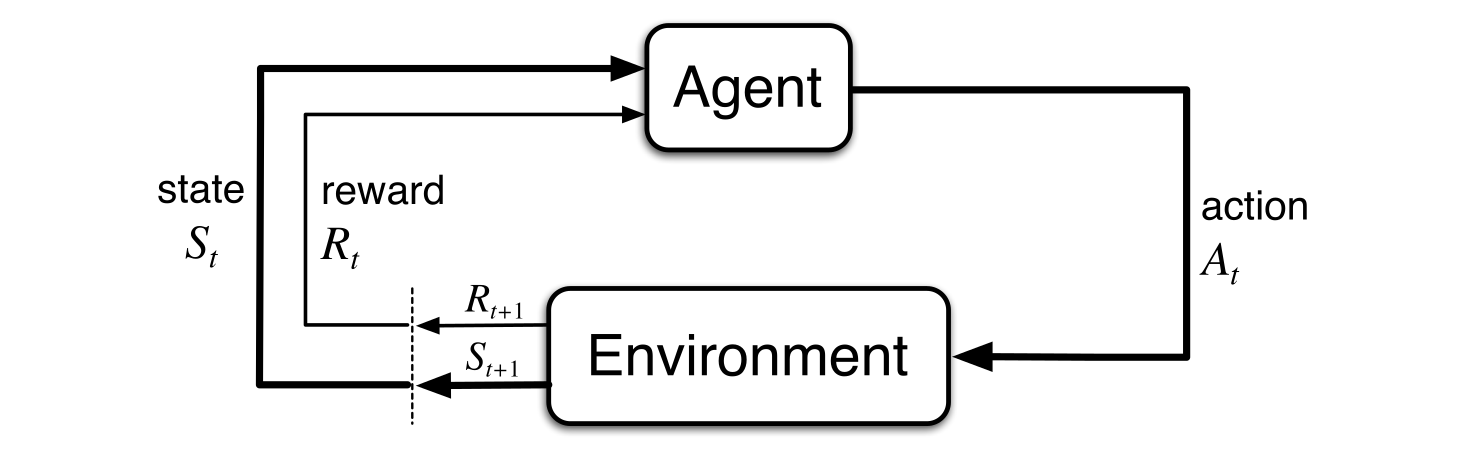
\includegraphics[width=0.9\textwidth]{imagenes/RL_Agent_Env.png}
    \caption{Interacción agente-entorno en proceso de decisión de Markov  (Sutton, R.S. and Barto, A.G (2020), p. 48).}
    \label{fig:agent_env_interaction}
\end{figure}

En los \textbf{MDPs finitos}, los conjuntos de estados, acciones y recompensas (\(\mathcal{S}\), \(\mathcal{A}\) y \(\mathcal{R}\)) contienen un número finito de elementos. Las variables aleatorias \(R_t\) y \(S_t\) siguen una distribución de probabilidad discreta \(p\), la cual depende únicamente del estado y la acción precedentes. Esta dependencia exclusiva se conoce como la propiedad de Markov, y para las metodologías a utilizar se asume el cumplimiento de esta.

\[
p(s',r|s,a) = \Pr\{ S_t=s', R_t=r | S_{t-1} = s, A_{t-1}=a \}
\]

Existen métodos que intentan desarrollar un modelo para comprender el entorno. Estos métodos intentan aprender esta función de probabilidad $p$ para poder planificar, y se les dice \textit{basados-en-modelo}. Por otro lado, tenemos los algoritmos \textit{libres-de-modelo} que buscan aprender las consecuencias de las acciones a través de la experiencia. Esto lo hacen sin estimar la función $p$, y son el grupo de algoritmos de interés para este trabajo.

\subsection{Retorno}
Como se dijo, el objetivo del agente es maximizar la recompensa acumulada recibida durante toda la ejecución. En general, buscamos maximizar el retorno esperado, donde el \textbf{retorno}, denotado $G_t$, se define como una función específica de una secuencia de recompensas. En el caso más simple, el retorno es la suma de las recompensas:

\[
G_t = R_{t+1} + R_{t+2} + R_{t+3} + \ldots + R_T,
\]

donde $T$ es el paso de tiempo final.

En muchos casos se debe destacar la fortaleza que tienen las recompensas más lejanas (en el tiempo) frente a las recompensas inmediatas, para esto usamos un \textit{factor de descuento} $\gamma$. El factor de descuento $\gamma$ es un parámetro, $0 \leq \gamma \leq 1$, y lo usamos para obtener el \textbf{retorno descontado}:

\[
G_t = R_{t+1} + \gamma R_{t+2} + \gamma^2 R_{t+3} + \ldots = \sum_{t=0}^{T} R_{t+1}
\]

\subsection{Función de acción-valor y política}
Todo algoritmo de RL involucra estimar una \textbf{función de valor}, la cual nos indica que "tan bueno" es que el agente esté en un determinado estado, o que tan bueno sea elegir cierta acción en un determinado estado. La noción de que "tan bueno" se define en términos de recompensas futuras esperadas. Las funciones de valor se definen con respecto a las formas particulares de actuar, llamadas políticas.

Una \textbf{política} es una función que mapea desde los estados a las probabilidades de seleccionar cada acción posible. Si el agente sigue una política $\pi$ en el instante de tiempo $t$, entonces $\pi(a|s)$ es la probabilidad de que $A_t=a$ si $S_t=s$.

La \textbf{función de valor} de un estado $s$ bajo una política $\pi$, denotada $V_{\pi}(s)$, es el retorno esperado al comenzar desde $s$ y siguiendo la política $\pi$ luego. Por otro lado, tenemos la \textbf{función de acción-valor} al elegir una acción $a$ en el estado $s$ bajo una política $\pi$, denotada \textbf{$Q_{\pi}(s,a)$}, que se define formalmente de la siguiente manera:

\[
Q_{\pi}(s,a) = \mathbb{E} \left[ G_t \mid S_t = s, A_t = a \right] = \mathbb{E} \left[ \sum_{t=0}^{T} R_{t+1} \mid S_t = s, A_t = a \right]
\]

Tanto $V_{\pi}$ como $Q_{\pi}$ pueden ser estimados desde la experiencia. Estas funciones se usan para definir una ordenación parcial sobre las políticas. Una política $\pi$ es mejor que $\pi'$ si su retorno esperado es mayor o igual, para todos los estados. Siempre hay al menos una política que es mejor o igual que otras políticas. A esta la llamamos \textbf{política óptima}, y la denotamos con $\pi_{*}$. Las políticas óptimas comparten la misma función estado-valor $V_{*}(s)$ y la misma función acción-valor $Q_{*}(s,a)$. Para nuestra solución, nos interesa esta última.


\subsection{Q-learning}
Una propiedad fundamental de $Q_*$ es que debe satisfacer la siguiente ecuación:

\[
Q_* (s,a) = \mathbb{E} \left[ R_{t+1} + \gamma \max_{a'} Q_*(S_{t+1},a') \mid S_t = s, A_t = a \right].
\]

Esta se llama \textbf{ecuación de optimalidad de Bellman} y es la base del algoritmo Q-learning. Utilizando esta ecuación como base y utilizando programación dinámica, obtenemos el siguiente método para aproximar $Q_*$:

\[
Q(S_t, A_t) \leftarrow Q(S_t, A_t) + \alpha \left[ R_{t+1} + \gamma \max_{a} Q_*(S_{t+1},a) - Q(S_t, A_t) \right].
\]

Donde \(\alpha\) es la \textit{tasa de aprendizaje}, un parámetro que controla la rapidez con la que los valores de \(Q\) convergen hacia los óptimos. Este proceso se repite hasta que los valores de \(Q\) converjan o hasta que se alcance un cierto número de iteraciones.

Para almacenar las aproximaciones de los valores Q utilizamos una tabla, llamada Q-table la cual contiene, en cada celda, la utilidad para todos los pares estado-acción.  Una vez que entrenamos a nuestro agente, y obtenemos una Q-table que aproxima lo suficientemente bien la función Q óptima, en consecuencia obtenemos una aproximación de la política óptima.

\subsection{Deep Learning}
Deep learning es un sub-campo específico de machine learning: una forma de aprender representaciones a partir de datos que hace hincapié en aprender sucesivas capas de representaciones cada vez más significativas. El ``deep'' en deep learning representa esta idea de capas sucesivas de representaciones. La cantidad de capas que contribuyen a un modelo de los datos se llama la profundidad del modelo. 

En deep learning, estas representaciones en capas se aprenden a través de modelos llamados redes neuronales (neural networks), estructuradas en capas apiladas unas sobre otras. Una red neuronal es un sistema de procesamiento de información diseñado para aprender y realizar tareas complejas a partir de datos de entrada. Una red neuronal está compuesta por un gran número de unidades de procesamiento, llamadas neuronas artificiales, que luego se interconectan.

Una neurona artificial consta de tres componentes principales:

\begin{enumerate}
    \item \textbf{Entradas}: Las neuronas reciben múltiples señales de entrada, cada una con un peso asociado que determina la importancia de esa entrada. Matemáticamente, las entradas se denotan como \(x1,x2,…,xn\) y los pesos asociados como \(w1,w2,…,wn\).

    \item \textbf{Función de Agregación}: La neurona combina las entradas ponderadas mediante una suma ponderada. Esto se puede expresar como:
    
    \[z = \sum_{i=1}^{n} w_i x_i + b\]

    donde \(b\) es el sesgo (bias), un término adicional que permite ajustar la salida de la neurona independientemente de las entradas.

    \item \textbf{Función de Activación}: La suma ponderada \(z\) se pasa a través de una función de activación para introducir no linealidad en el modelo, lo que permite a la red neuronal aprender y representar relaciones complejas. Algunas funciones de activación comunes son:
    \begin{itemize}
        \item \textbf{Sigmoide}: \(\sigma(z) = \frac{1}{1 + e^{-z}}\)
        
        \item \textbf{Tangente hiperbólica (tanh)}: \(\text{tanh}(z) = \frac{e^z - e^{-z}}{e^z + e^{-z}}\)
        
        \item \textbf{ReLU (Rectified Linear Unit)}: \(\text{ReLU}(z) = \max(0, z)\)
        
        \item \textbf{Softmax}: Normaliza un vector de valores reales en una distribución de probabilidad. Es ampliamente utilizada en la capa de salida de modelos de clasificación multiclase. Se define como:
        \[
        \text{Softmax}(z_i) = \frac{e^{z_i}}{\sum_{j=1}^{K} e^{z_j}}
        \]
        donde \(K\) es el número de clases posibles.
        
        \item \textbf{Gumbel-Softmax}: Es una extensión diferenciable de la función \textit{Softmax}, utilizada para muestrear variables categóricas de manera continua y diferenciable, lo que permite el entrenamiento mediante retropropagación. Se define como:
        \[
        y_i = \frac{\exp\left((\log(\pi_i) + g_i)/\tau\right)}{\sum_{j=1}^{K} \exp\left((\log(\pi_j) + g_j)/\tau\right)}
        \]
        donde \(g_i\) son variables aleatorias Gumbel (\(g_i = -\log(-\log(u_i))\), con \(u_i \sim \text{Uniform}(0,1)\)), \(\pi_i\) son las probabilidades de clase, y \(\tau > 0\) es el parámetro de temperatura que controla la suavidad de la aproximación.
    \end{itemize}
\end{enumerate}

\subsubsection{Funcionamiento de una neurona artificial}

\begin{enumerate}
\item \textbf{Recepción de Entradas}: La neurona recibe las entradas \(x1,x2,…,xn\) de la capa anterior de la red o directamente de los datos de entrada.

\item \textbf{Agregación de Entradas Ponderadas}: Cada entrada se multiplica por su peso correspondiente y se suman todas las entradas ponderadas junto con el sesgo \(b\).

\item \textbf{Aplicación de la Función de Activación}: La suma ponderada \(z\) se pasa a través de la función de activación para producir la salida de la neurona \(a\).

\item \textbf{Propagación de la Salida}: La salida \(a\) se envía a las neuronas de la siguiente capa en la red neuronal.
\end{enumerate}

\subsubsection{Deep Reinforcement Learning}

El Deep Reinforcement Learning (DRL) es una sub-área del aprendizaje profundo que combina las técnicas de aprendizaje profundo con el aprendizaje por refuerzo (reinforcement learning, RL). En el DRL, las redes neuronales profundas se utilizan para aproximar funciones de valor o políticas, permitiendo que los agentes de RL puedan tomar decisiones en entornos complejos y de alta dimensionalidad.

El DRL ha demostrado ser efectivo en una variedad de aplicaciones, desde juegos (como el Go, donde el algoritmo AlphaGo superó a jugadores humanos profesionales) hasta la robótica y el control de sistemas autónomos. La combinación de deep learning y RL permite a los agentes aprender estrategias complejas y adaptativas, superando las limitaciones de los enfoques tradicionales de RL. 

\subsection{Deep Q-Learning}
Cuando el espacio de estados y de acciones no es suficientemente chico, el algoritmo Q-learning no es apropiado para manejar el problema de encontrar una política óptima. Cuando hay millones de estados posibles, la tabla se vuelve enorme, y no es viable su utilización. En otras palabras, no es escalable. 

Una forma de solventar el problema de escalabilidad es combinar Q-learning con redes neuronales profundas. Este enfoque se conoce como Deep Q-learning (DQL). La redes neuronales en DQL actúan como aproximadores de los valores Q para cada par estado-acción. La red neuronal recibe un estado como entrada y devuelve los valores Q para todas las posibles acciones. En la \autoref{fig:dql_vs_ql} se ilustra la diferencia principal entre Q-learning y deep Q-learning al evaluar los valores Q.

\begin{figure}
    \centering
    \includegraphics[width=0.9\linewidth]{.imagenes/Q-learning vs Deep Q-learning}
    \caption{Q-learning vs Deep Q-learning. Imagen extraída de \textit{From Q-Learning to Deep Q-Learning - Hugging Face Deep RL Course} \cite{huggingface_dqn}}
    \label{fig:dql_vs_ql}
\end{figure}

Adicionalmente, el aprendizaje obtenido de un estado, mediante redes neuronales, se transfiere a estados similares, por lo que se podrán hacer buenas estimaciones para estados que no han sido visitados con anterioridad.

\subsubsection{Target network}
Deep Q-learning usa dos redes neuronales para el proceso de aprendizaje. La primera, la red neuronal principal (main network), representada por los parámetros \(\theta\), la cual se utiliza para estimar los valores. Luego tenemos la segunda, la red objetivo (target network), parametrizada por \(\theta'\), la cual tendrá la misma arquitectura que la red principal pero se usará para aproximar los valores Q del siguiente estado \(s'\) y la siguiente acción \(a'\). El aprendizaje ocurre en la red principal y no en la objetivo. La red objetivo no cambia sus parámetros durante varias iteraciones, y después los parámetros de la red principal se copian a la red objetivo, transmitiendo así el aprendizaje de una a otra, haciendo que las estimaciones calculadas por la red objetivo sean más precisas.

\subsubsection{Experience replay}
Interactuar con el entorno para obtener información sobre el impacto de las acciones tiene un coste. Si al obtener información la desechamos tras usarla, estamos perdiendo la oportunidad de volver a utilizarla en el futuro. Para aprovechar mejor la información obtenida, usamos una técnica llamada \textit{experience replay}, la cual almacena la experiencia obtenida en un \textit{buffer} de tamaño determinada. Esta experiencia se representa como la tupla conformada por el estado, la acción, la recompensa obtenida y el estado siguiente \((s,a,r,s')\). 

Deep Q-learning usa \textit{experience replay} para aprender en pequeños \textit{batches}, para evitar sesgar la distribución del conjunto de datos de los diferentes estados, acciones, recompensas y estados siguientes que verá la red neuronal. La razón por la cual se utiliza esta técnica, es para eliminar la correlación que surge cuando entrenamos en experiencias que suceden una junto después de la otra. Al entrenar aleatoriamente sobre diferentes situaciones en momentos diferentes, somos capaces de aprender de forma más objetiva que acciones se correlacionan realmente con un valor Q alto.

\subsubsection{Ecuación de Bellman en DQN}

La ecuación de Bellman es fundamental en los métodos de aprendizaje por refuerzo. En el contexto de Deep Q-Networks (DQN), la ecuación de Bellman se adapta para actualizar los valores Q estimados por la red neuronal. La ecuación de Bellman en DQN tiene la siguiente forma:


\[
Q(s, a; \theta) = r + \gamma \max_{a'} Q(s', a'; \theta^{-})
\]


donde \( Q(s, a; \theta) \) es el valor Q estimado para el estado \( s \) y la acción \( a \) con los parámetros actuales de la red neuronal principal, \( r \) es la recompensa obtenida, \( \gamma \) es el factor de descuento, y \( \max_{a'} Q(s', a'; \theta^{-}) \) es el valor Q máximo estimado para el siguiente estado \( s' \) con los parámetros de la red objetivo.

Para entrenar una red neuronal utilizando DQN, necesitamos definir una función de pérdida (\textit{loss function}). La función de pérdida en DQN se define como el cuadrado de la diferencia entre ambos lados de la ecuación de Bellman. Esta pérdida se minimiza durante el proceso de entrenamiento para ajustar los pesos de la red neuronal. La función de pérdida se expresa como:

\begin{equation}
\mathcal{L}(\theta) = \mathbb{E} \left[ \left( r + \gamma \max_{a'} Q(s', a'; \theta^{-}) - Q(s, a; \theta) \right)^2 \right]
\end{equation}

donde \(\theta\) representa los parámetros actuales de la red neuronal principal y \(\theta^{-}\) representa los parámetros de la red objetivo (target network), que se actualizan periódicamente.

\subsubsection{Algoritmo DQL con \textit{experience replay}}
El algoritmo deep Q-learning consta de dos fases: muestreo y entrenamiento. Durante el sampling se realizan acciones y se almacenan las tuplas de experiencia en el \textit{replay buffer}. En la fase entrenamiento se selecciona un pequeño \textit{batch} de tuplas, de forma aleatoria, y se aprende de este \textit{batch} utilizando un paso de actualización por descenso de gradiente.

\begin{algorithm}
    \caption{Deep Q-Network with Experience Replay} 
    \begin{algorithmic}[1]
        \State Initialize replay memory $D$ to capacity $N$
        \State Initialize action-value function $Q$ with random weights $\theta$
        \State Initialize target action-value function $\hat{Q}$ with weights $\theta^- = \theta$
        \For {$episode = 1, 2, \ldots$}
            \State Initialize sequence $s_1 = \{x_1\}$ and preprocessed sequence $\phi_1 = \phi(s_1)$
            \For {$t = 1, 2, \ldots, T$}
                \State With probability $\epsilon$ select random action $a_t$
                \State Otherwise select $a_t = \argmax_a Q(\phi(s_t), a; \theta)$
                \State Execute action $a_t$ in emulator and observe reward $r_t$ and image $x_{t+1}$
                \State Set $s_{t+1} = s_t, a_t, x_{t+1}$ and preprocess $\phi_{t+1} = \phi(s_{t+1})$
                \State Store transition $(\phi_t, a_t, r_t, \phi_{t+1})$ in $D$
                \State Sample random minibatch of transitions $(\phi_j, a_j, r_j, \phi_{j+1})$ from $D$
                \State Set $y_j = r_j + \gamma \max_{a'} \hat{Q}(\phi_{j+1}, a'; \theta^-)$ (use $r_j$ for terminal $\phi_{j+1})$
                \State Perform gradient descent step on $(y_j - Q(\phi_j, a_j; \theta))^2$ with respect to $\theta$
                \State Every C steps reset $\hat{Q} = Q$
            \EndFor
        \EndFor
    \end{algorithmic} 
\end{algorithm}

\newpage


\subsubsection{PPO}

\subsubsection{DDPG}

\subsection{Exploración vs. Explotación}

En un problema de \textit{reinforcement learning} es importante lograr un buen balance entre la \textbf{exploración} del espacio de acciones ante un estado determinado, y la \textbf{explotación} de las acciones que otorgan una mejor recompensa. Es importante realizar una buena exploración del entorno, ya que sino es posible que el agente se atasque en un óptimo local. Tampoco hay que excederse en la exploración, ya que esto produce una recompensa acumulada baja.

Una de las estrategias de exploración más utilizadas es $\epsilon$-greedy. En Q-learning, se selecciona una acción basada en la recompensa esperada. El agente siempre elige la acción óptima, de forma tal que se maximice el retorno desde el estado actual. Si seguimos una política $\epsilon$-greedy, para seleccionar la próxima acción, el agente seleccionará la acción que maximice la recompensa con una probabilidad de $1-\epsilon$. Caso contrario, elegirá una acción de forma aleatoria.

\[
a = 
\begin{cases} 
    \max_{a} Q(s,a) & \text{con probabilidad } 1 - \epsilon  \\
    \text{aleatoria} & \text{caso contrario}
\end{cases}
\]

A medida que se progresa en los episodios de entrenamiento del agente, el valor de $\epsilon$ disminuye, lo que resulta en una reducción de la exploración conforme nos acercamos a los últimos episodios de entrenamiento. Para nuestro problema, se decidió utilizar un decaimiento lineal de $\epsilon$ hasta alcanzar una fracción específica del entrenamiento, momento en el cual $\epsilon$ se mantiene constante en un valor mínimo hasta el final del proceso de aprendizaje, como se muestra en la  \autoref{fig:epsilonLinearDecay}.

% \begin{figure}
%     \centering
%     \includegraphics[width=1.0\linewidth]{imagenes/}
%     \caption{Función de caída lineal de epsilon durante 200 episodios. Con un $\epsilon$ inicial igual a 1, $\epsilon$ final igual a 0.01,  y un factor de exploración de 0.7.}
%     \label{fig:epsilonLinearDecay}
% \end{figure}



\subsection{Aprendizaje por Refuerzo Multi-Agente Cooperativo (MARL)}
\label{subsec:marl_cooperativo}

El \textbf{aprendizaje por refuerzo multi-agente} (en inglés, \emph{Multi-Agent Reinforcement Learning}, abreviado \textbf{MARL}) extiende el paradigma del aprendizaje por refuerzo (RL, por sus siglas en inglés, \emph{Reinforcement Learning}) al caso en el que existen múltiples agentes que aprenden e interactúan simultáneamente dentro de un mismo entorno.  
A diferencia del aprendizaje por refuerzo clásico, donde un único agente aprende una política óptima para maximizar su recompensa esperada, en MARL cada agente influye en la dinámica del entorno a través de sus acciones, lo que genera interdependencias complejas y desafíos adicionales de coordinación, asignación de crédito y estabilidad del aprendizaje.  
Cuando los agentes comparten un objetivo común, se habla de un \textbf{entorno cooperativo}, que es el caso de estudio de este trabajo. \cite{marlbook}

\subsubsection{Formalización mediante Dec-POMDP}
Un marco formal ampliamente utilizado para modelar problemas cooperativos de este tipo es el \textbf{Decentralized Partially Observable Markov Decision Process} (\textbf{Dec-POMDP}, por sus siglas en inglés).  
Un Dec-POMDP para $n$ agentes se define como una tupla:
\[
\langle \mathcal{S}, \{ \mathcal{A}_i \}_{i=1}^n, T, R, \{ \Omega_i \}_{i=1}^n, O, \gamma \rangle,
\]
donde:
\begin{itemize}
  \item $\mathcal{S}$ representa el conjunto de estados globales del entorno.
  \item $\mathcal{A}_i$ es el conjunto de acciones disponibles para el agente $i$.
  \item $T(s' \mid s, a_1, \dots, a_n)$ es la función de transición de estados, que determina la probabilidad de pasar de un estado $s$ a un nuevo estado $s'$ dadas las acciones conjuntas de todos los agentes.
  \item $R(s, a_1, \dots, a_n)$ es la función de recompensa, compartida entre los agentes en entornos cooperativos.
  \item $\Omega_i$ es el conjunto de observaciones posibles para el agente $i$, y $O(o_1, \dots, o_n \mid s', a_{1:n})$ es la función de observación, que describe qué observa cada agente tras una transición.
  \item $\gamma \in [0,1)$ es el factor de descuento temporal.
\end{itemize}

En cada instante de tiempo $t$, cada agente $i$ selecciona una acción $a_i$ según su política \emph{descentralizada} $\pi_i(a_i \mid \tau_i)$, donde $\tau_i$ representa la historia o secuencia de observaciones locales del agente.  
El objetivo global del sistema es maximizar el retorno conjunto esperado:
\[
J(\pi_{1:n}) = \mathbb{E}\!\left[ \sum_{t=0}^{\infty} \gamma^t R(S_t, A_{1,t}, \dots, A_{n,t}) \right].
\]
Esta formulación provee la base matemática sobre la cual se desarrollan los algoritmos modernos de MARL. \cite{decpomdp-survey,marlbook}

\subsection{Paradigma CTDE: Entrenamiento Centralizado con Ejecución Descentralizada}
Una estrategia ampliamente adoptada en entornos cooperativos es el esquema \textbf{Centralized Training with Decentralized Execution} (\textbf{CTDE}), es decir, \emph{entrenamiento centralizado con ejecución descentralizada}.  
Bajo este paradigma, los agentes pueden acceder a información global (por ejemplo, el estado completo del entorno o las acciones de todos los agentes) durante la fase de entrenamiento, pero durante la ejecución cada uno actúa únicamente con su información local.  
Este enfoque equilibra la eficiencia del aprendizaje con la factibilidad práctica de la ejecución descentralizada, lo cual resulta fundamental en entornos reales como el control del tráfico urbano. \cite{ctde_survey,marlbook}

\subsection{Principales Familias de Algoritmos Cooperativos}

\paragraph{Descomposición de valores (VDN y QMIX).}
El enfoque de \textbf{Value Decomposition Networks} (VDN) propone descomponer la función de valor conjunta $Q_{\text{tot}}$ en una suma de valores individuales por agente:
\[
Q_{\text{tot}}(\tau, a) \approx \sum_i Q_i(\tau_i, a_i),
\]
lo que permite aprender políticas locales manteniendo un objetivo global coherente.  
\textbf{QMIX}, por su parte, generaliza esta idea utilizando una red de mezcla que combina los valores locales $Q_i$ condicionada al estado global, imponiendo una restricción de monotonía que asegura que la acción conjunta óptima pueda derivarse de las mejores acciones individuales. \cite{vdn,qmix}

\paragraph{Métodos actor-crítico centralizados (COMA y MADDPG).}
En los métodos del tipo \textbf{actor-crítico}, cada agente mantiene una política parametrizada (actor) y un estimador del valor esperado (crítico).  
En entornos cooperativos se introducen críticos \emph{centralizados}, que tienen acceso a información global, mientras que los actores permanecen descentralizados:
\begin{itemize}
  \item \textbf{COMA} (\emph{Counterfactual Multi-Agent Policy Gradient}) introduce un \emph{baseline contrafactual} que mide la contribución marginal de cada agente a la recompensa global, facilitando la asignación de crédito. \cite{coma}
  \item \textbf{MADDPG} (\emph{Multi-Agent Deep Deterministic Policy Gradient}) extiende el algoritmo DDPG al contexto multi-agente, empleando un crítico centralizado por agente que considera las acciones de todos los demás, y es adecuado para espacios de acción continuos. \cite{maddpg}
\end{itemize}




\paragraph{MADDPG}

El algoritmo \textit{Multi-Agent Deep Deterministic Policy Gradient} (MADDPG), propuesto por Lowe et al. \cite{lowe2017maddpg}, extiende el método DDPG al contexto multiagente mediante el paradigma de \textit{aprendizaje centralizado con ejecución descentralizada} (\textit{Centralized Training with Decentralized Execution}, CTDE). En este enfoque, cada agente aprende una política determinista individual que se actualiza utilizando información global disponible solo durante el entrenamiento, como los estados y acciones de todos los agentes. Durante la ejecución, en cambio, cada agente actúa basándose únicamente en sus propias observaciones locales.

MADDPG utiliza una red crítica centralizada para cada agente, que estima la función de valor de acción \(Q_i(s, a_1, \dots, a_N)\) considerando las acciones conjuntas del entorno multiagente, y una red de política (actor) descentralizada \(\mu_i(o_i)\) que determina la acción óptima a partir de la observación local \(o_i\). De esta forma, el método mitiga la no estacionariedad inherente a los entornos multiagente y mejora la estabilidad del entrenamiento, permitiendo a los agentes aprender comportamientos cooperativos o competitivos de manera eficiente en entornos continuos.


\paragraph{Técnicas de modelado de recompensas.}
La \textbf{asignación de crédito} consiste en determinar cuánto contribuye cada agente al desempeño global.  
Se han propuesto distintos mecanismos para abordarla:
\begin{itemize}
  \item \emph{Difference rewards} (\(D_i = G - G_{\setminus i}\)): miden la diferencia en el retorno total si el agente $i$ no hubiese actuado.
  \item \emph{Reward shaping} basado en funciones potenciales, que ajusta las recompensas individuales sin alterar el óptimo global. \cite{difference_rewards}
\end{itemize}

\subsection{Desafíos prácticos en MARL}

\paragraph{No estacionariedad.}
El entorno percibido por cada agente cambia constantemente mientras los demás actualizan sus políticas, lo que viola el supuesto de estacionariedad clásico del aprendizaje por refuerzo.  
Para mitigar este problema se aplican estrategias como:
\begin{itemize}
  \item Entrenamiento centralizado (CTDE).
  \item Inclusión de \emph{fingerprints} o identificadores de versión de política en las muestras del \emph{replay buffer}.
  \item Muestreo ponderado por importancia o eliminación de experiencias obsoletas. \cite{foerster2017}
\end{itemize}

\paragraph{Almacenamiento y reutilización de experiencias.}
El uso del \textbf{replay buffer} (memoria de experiencias) en MARL requiere especial cuidado, ya que las transiciones antiguas pueden volverse inconsistentes con las políticas actuales. Se aplican técnicas de etiquetado temporal o ponderación adaptativa para mantener la estabilidad del aprendizaje. \cite{foerster2017}

\paragraph{Escalabilidad.}
En escenarios con gran número de agentes, como redes urbanas de tráfico, la complejidad crece rápidamente. Para enfrentar este problema se utilizan:
\begin{itemize}
  \item \textbf{Parameter sharing} (compartición de parámetros) entre agentes homogéneos.
  \item \textbf{Arquitecturas de redes neuronales de grafos} (GNN, por sus siglas en inglés), que aprovechan la estructura espacial de la red vial y permiten intercambiar información entre intersecciones vecinas. \cite{gnn_traffic}
\end{itemize}


\subsection{Terminología utilizada}

A continuación se dan las definiciones de terminología importante a la hora de explicar la solución propuesta y discutir los resultados. Todas las definiciones incluidas fueron extraídas de la presentación realizada por Hua Wei, Zhenhui Li y Vikash Gayah en IEEE ITSC‘20 Tutorial \cite{HW2020DRLTSCSlidesIEEE}, y de la documentación de SUMO \cite{sumo-doc}.

\textbf{Carril} (\textit{lane}): Una intersección está compuesta por un conjunto de carriles. Hay dos tipos de carriles: carriles entrantes y carriles salientes. Como se muestra en la \autoref{intersectionElements}.

\textbf{Enlace} (\textit{link}): Un enlace es una conexión entre carriles. Define los posibles movimientos en un carril, tales como avanzar, girar a la izquierda o a la derecha. Como se muestra en la \autoref{intersectionElements}.

\begin{figure}[H]
    \centering
    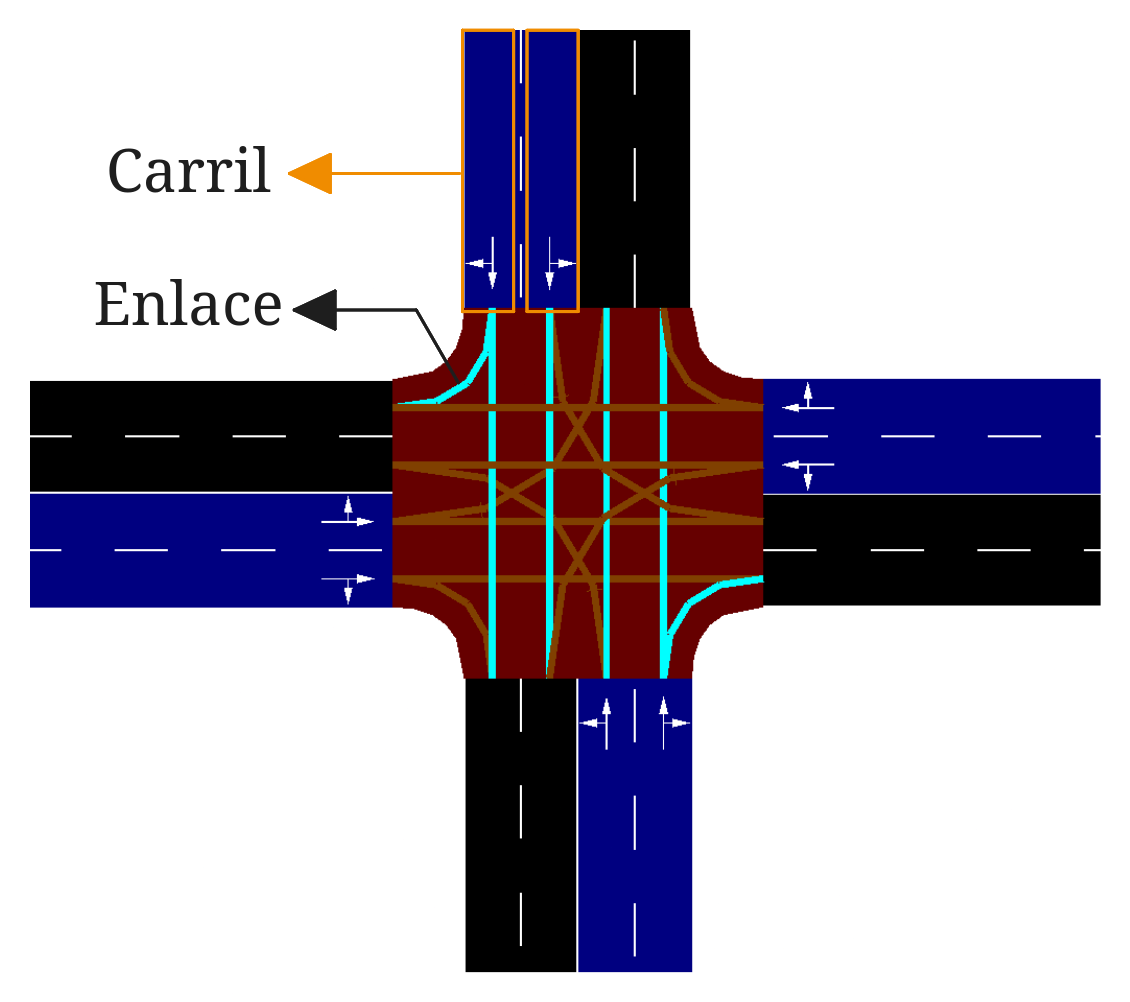
\includegraphics[width=0.8\textwidth]{./imagenes/intersectionElements.png}
    \caption{Carriles y enlaces. En azul se indican los carriles entrantes y en negro los salientes.}
    \label{intersectionElements}
\end{figure}

\textbf{Señal de movimiento}: Una señal de movimiento define cómo se debe circular el tráfico. Un carril puede contener varias señales de movimiento; por ejemplo, en el carril izquierdo puede existir una señal que permita girar a la izquierda y otra para continuar recto. Estas señales son provistas por los semáforos y, mediante un color, indican las restricciones de movimiento. Los colores utilizados son:

\begin{itemize}
    \item \textbf{Rojo}: movimiento no permitido; los vehículos deben detenerse.
    \item \textbf{Amarillo}: el movimiento será restringido en $X$ segundos; los vehículos deben desacelerar si están lejos de la intersección.
    \item \textbf{Verde oscuro (sin prioridad)}: movimiento permitido solo si no se aproximan vehículos con prioridad.
    \item \textbf{Verde claro (con prioridad)}: movimiento permitido, con prioridad de paso.
\end{itemize}

\textbf{Fase}: Una fase es una combinación de señales de movimiento que define el estado de un semáforo en un instante determinado. En la \autoref{trafficSignals} se observa un ejemplo de fase en una intersección de cuatro carriles.

\begin{figure}[H]
    \centering
    
\includegraphics[width=0.7\textwidth]{./Images/trafficSignals.png}
    \caption{Semáforo en la fase ``GrGr''. La letra ``G'' indica luz verde para el enlace 0, seguida de la roja para el enlace 1, verde para el enlace 2 y roja para el enlace 3.}
    \label{trafficSignals}
\end{figure}

\textbf{Intervalo}: Período de tiempo durante el cual las señales de una fase permanecen constantes.

\textbf{Secuencia de fases}: Conjunto ordenado de fases y sus respectivos intervalos, que define la programación completa de un semáforo.

\textbf{Tiempo de espera de un vehículo}: En el contexto del simulador SUMO, se define como el tiempo (en segundos) durante el cual un vehículo mantiene una velocidad inferior a 0.1 m/s (detención) desde la última vez que superó dicho valor. El contador se reinicia cada vez que el vehículo vuelve a moverse.

\textbf{Tiempo de espera acumulado de un vehículo}: Tiempo total (en segundos) durante el cual un vehículo ha permanecido detenido (velocidad < 0.1 m/s) a lo largo de toda la simulación.

\textbf{Zona de asignación de tráfico} (\textit{Traffic Assignment Zone, TAZ}): Representa una unidad espacial utilizada para definir el origen y destino de los flujos vehiculares dentro de la red. Cada TAZ agrupa un conjunto de nodos o arcos de la red y sirve como punto lógico de entrada o salida del tráfico. Las TAZ se emplean para generar matrices origen-destino (O/D) y permiten modelar la demanda de viajes de forma agregada \cite{sumo-doc}.

\textbf{Matriz Origen-Destino (O/D)}: Estructura de datos que especifica la cantidad de viajes que se generan desde una TAZ de origen hacia una TAZ de destino en un intervalo de tiempo determinado. En SUMO, las matrices O/D se utilizan para construir rutas y definir la demanda vehicular mediante asignación de tráfico.

\textbf{Ruta} (\textit{route}): Secuencia de arcos o carriles que sigue un vehículo desde su origen hasta su destino. Las rutas pueden ser estáticas (predefinidas) o dinámicas (ajustadas durante la simulación mediante algoritmos de asignación).

\textbf{Tipo de vehículo} (\textit{vehicle type}): Conjunto de atributos que definen el comportamiento y características físicas de un vehículo, tales como longitud, aceleración, velocidad máxima, color, tipo de conductor o clase de prioridad.

\textbf{Flujo} (\textit{flow}): Define un conjunto de vehículos con características similares que ingresan a la red siguiendo un mismo patrón de generación temporal y espacial. Es una forma simplificada de especificar la demanda sin detallar cada vehículo individualmente.

\textbf{Demanda de tráfico} (\textit{traffic demand}): Conjunto de rutas, vehículos y flujos que representan el volumen de tráfico simulado en un escenario determinado. Su correcta definición es esencial para reproducir condiciones realistas de tránsito urbano.
